\documentclass[11pt]{article}
\usepackage[notes]{la}
\lamodule{6}{7}{Inner Product Spaces}
\laxdoc{4.1}
\laxdoc{6.1}
\laxdoc{6.2}
\laxdoc{6.3}
\laxdoc{6.4}

\begin{document}

\section{Inner Product Spaces}

\begin{guide}
In this chapter the dot product gave us length, distance, perpendicular vectors, projections and best approximations. But look at what the proofs actually used. They used a few rules: the dot product is symmetric, it respects sums and scalar multiples, and $\bv{u}\cdot\bv{u}$ is positive unless $\bv{u}=\bv{0}$. They never used the fact that a vector is a column of numbers. This section takes that observation seriously. Any rule $\inner{\bv{u}}{\bv{v}}$ with those properties, on any vector space from Section 4.1, is called an \emph{inner product}, and then everything we proved about lengths, orthogonality, Gram--Schmidt and best approximation holds again, with the same proofs. The payoff is that we can talk about the length of a polynomial, about two functions being perpendicular, and about the \emph{best polynomial approximation of a function}.
\end{guide}

\textbf{By the end of this section you should be able to:}
\begin{itemize}
  \item state the four rules of an inner product and decide whether a given rule satisfies them;
  \item compute lengths, distances and inner products in $\R^n$ with a weighted dot product, and in spaces of polynomials and functions with an integral;
  \item prove the basic rules, the Cauchy--Schwarz inequality and the triangle inequality from the four rules alone;
  \item apply the Gram--Schmidt process in an inner product space;
  \item find the best approximation of a vector, for instance a function, by a subspace, and compute the error.
\end{itemize}

% ---------------------------------------------------------------------
\subsection*{Which rules does the dot product really use?}

\begin{defn}{Inner product}{ip}
Let $V$ be a vector space (Definition~\ref{4.1-def:vspace}). An \emph{inner product} on $V$ is a rule that assigns to every pair of vectors $\bv{u},\bv{v}$ in $V$ a real number $\inner{\bv{u}}{\bv{v}}$ such that, for all $\bv{u},\bv{v},\bv{w}$ in $V$ and every scalar $c$:
\begin{enumerate}[label=(\arabic*),itemsep=1pt]
  \item $\inner{\bv{u}}{\bv{v}}=\inner{\bv{v}}{\bv{u}}$ \hfill (symmetry)
  \item $\inner{\bv{u}+\bv{v}}{\bv{w}}=\inner{\bv{u}}{\bv{w}}+\inner{\bv{v}}{\bv{w}}$ \hfill (additivity)
  \item $\inner{c\bv{u}}{\bv{v}}=c\,\inner{\bv{u}}{\bv{v}}$ \hfill (homogeneity)
  \item $\inner{\bv{u}}{\bv{u}}\ge0$, and $\inner{\bv{u}}{\bv{u}}=0$ only when $\bv{u}=\bv{0}$ \hfill (positive definiteness)
\end{enumerate}
A vector space with an inner product is an \emph{inner product space}. The dot product on $\R^n$ is an inner product (Theorem~\ref{6.1-thm:dotprops}); the point of this section is that it is not the only one.
\end{defn}

\begin{exmp}{A weighted dot product on $\R^2$}{weighted}
For $\bv{u}=(u_1,u_2)$ and $\bv{v}=(v_1,v_2)$ put $\inner{\bv{u}}{\bv{v}}=2u_1v_1+3u_2v_2$. Rules (1) to (3) hold because each is a statement about the numbers $u_1,u_2,v_1,v_2$ and a sum of two terms: for instance $\inner{c\bv{u}}{\bv{v}}=2(cu_1)v_1+3(cu_2)v_2=c(2u_1v_1+3u_2v_2)$. For rule (4), $\inner{\bv{u}}{\bv{u}}=2u_1^2+3u_2^2\ge0$, and it is $0$ only if $u_1=u_2=0$. So this is an inner product. Take $\bv{u}=(1,2)$ and $\bv{v}=(3,-1)$. Then
\[
\inner{\bv{u}}{\bv{v}}=2\cdot1\cdot3+3\cdot2\cdot(-1)=6-6=0,\qquad\text{while}\qquad\bv{u}\cdot\bv{v}=3-2=1 .
\]
The vectors $(1,2)$ and $(3,-1)$ are orthogonal for this inner product and not for the dot product. Their squared lengths are $\inner{\bv{u}}{\bv{u}}=2+12=14$ and $\inner{\bv{v}}{\bv{v}}=18+3=21$.
\end{exmp}

\begin{exmp}{Three rules that fail}{notip}
Each rule below is defined on $\R^2$, and each fails a different part of Definition~\ref{def:ip}.
\begin{itemize}
  \item $\inner{\bv{u}}{\bv{v}}=u_1v_1-u_2v_2$ fails (4) in its first part: $\inner{(0,1)}{(0,1)}=-1<0$.
  \item $\inner{\bv{u}}{\bv{v}}=u_1v_1$ fails the second part of (4): $\inner{(0,1)}{(0,1)}=0$ although $(0,1)\neq\bv{0}$.
  \item $\inner{\bv{u}}{\bv{v}}=|u_1v_1|+|u_2v_2|$ fails (3): with $c=-1$, $\bv{u}=\bv{v}=(1,0)$ we get $\inner{c\bv{u}}{\bv{v}}=1$ but $c\inner{\bv{u}}{\bv{v}}=-1$.
\end{itemize}
\end{exmp}

\begin{exmp}{Polynomials with an integral}{integral}
On $\mathbb{P}_2$, the polynomials of degree at most $2$, put
\[
\inner{p}{q}=\int_{-1}^{1}p(t)\,q(t)\,dt .
\]
Rule (1) holds because $p(t)q(t)=q(t)p(t)$, and rules (2) and (3) hold because an integral of a sum is the sum of the integrals and constants come out. For (4), $\inner{p}{p}=\int_{-1}^1p(t)^2\,dt\ge0$ because $p(t)^2\ge0$. If $p\neq0$, then $p(t_0)\neq0$ for some $t_0$ in $[-1,1]$, so $p(t)^2$ is positive on a small interval around $t_0$ (it is continuous), and the integral is positive. So $\inner{p}{p}=0$ forces $p=0$. This is an inner product. Since $\int_{-1}^1t^k\,dt=\frac{2}{k+1}$ for even $k$ and $0$ for odd $k$, the inner products of the powers are
\begin{center}
\begin{tabular}{c|ccc}
$\inner{\cdot}{\cdot}$ & $1$ & $t$ & $t^2$\\ \hline
$1$ & $2$ & $0$ & $\tfrac23$\\
$t$ & $0$ & $\tfrac23$ & $0$\\
$t^2$ & $\tfrac23$ & $0$ & $\tfrac25$
\end{tabular}
\end{center}
For $p=1-t$ and $q=2+3t$: $\inner{p}{q}=\int_{-1}^1(2+t-3t^2)\,dt=4+0-2=2$.
\end{exmp}

\begin{exmp}{A sum over three points}{evalip}
On $\mathbb{P}_2$ let $\inner{p}{q}=p(-1)q(-1)+p(0)q(0)+p(1)q(1)$. Rules (1) to (3) are clear. For (4), $\inner{p}{p}=p(-1)^2+p(0)^2+p(1)^2\ge0$. If it is $0$, then $p(-1)=p(0)=p(1)=0$; for $p(t)=a+bt+ct^2$ this says $a=0$, $a+b+c=0$ and $a-b+c=0$, hence $b=c=0$ and $p=0$. So this is an inner product on $\mathbb{P}_2$, different from the integral one. For $p=1-t$ and $q=2+3t$ the values at $-1,0,1$ are $(2,1,0)$ and $(-1,2,5)$, so $\inner{p}{q}=-2+2+0=0$: now $p$ and $q$ are orthogonal, whereas for the integral inner product $\inner{p}{q}=2$. Also $\inner{p}{p}=4+1+0=5$, against $\int_{-1}^1(1-t)^2\,dt=\tfrac83$.
\end{exmp}

\begin{exmp}{The same rule on a bigger space fails}{evalfail}
On $\mathbb{P}_3$ the same formula, $\inner{p}{q}=p(-1)q(-1)+p(0)q(0)+p(1)q(1)$, is \emph{not} an inner product. The polynomial $p(t)=t^3-t$ is not the zero polynomial, but $p(-1)=p(0)=p(1)=0$, so $\inner{p}{p}=0$, and rule (4) fails. Three values cannot detect every polynomial of degree $3$.
\end{exmp}

\begin{proc}{Is this rule an inner product?}{checkip}
\begin{enumerate}[nosep]
  \item Check that $\inner{\bv{u}}{\bv{v}}$ is a real number for all $\bv{u},\bv{v}$ in $V$.
  \item Symmetry (1): swap the two vectors and compare.
  \item Additivity (2) and homogeneity (3): expand the first slot. With symmetry this gives the same rules for the second slot.
  \item Positivity (4): write $\inner{\bv{u}}{\bv{u}}$ as a sum of squares or an integral of a square, so that $\ge0$ is clear.
  \item Definiteness (4): suppose $\inner{\bv{u}}{\bv{u}}=0$ and show $\bv{u}=\bv{0}$. This is the step that fails most often; try to find a nonzero $\bv{u}$ with $\inner{\bv{u}}{\bv{u}}=0$ before you try to prove it.
\end{enumerate}
\end{proc}

\begin{think}{Why this much?}{noneg}
In Example~\ref{ex:notip}, the rule $u_1v_1-u_2v_2$ gives $\inner{(0,1)}{(0,1)}=-1$. What would the ``length'' $\sqrt{\inner{\bv{u}}{\bv{u}}}$ of $(0,1)$ be? Which part of Definition~\ref{def:ip} protects us from this?
\end{think}

\begin{kc}{Compute with a weighted dot product}{kcweight}
With $\inner{\bv{u}}{\bv{v}}=2u_1v_1+3u_2v_2$ as in Example~\ref{ex:weighted}, compute $\inner{(2,1)}{(1,-2)}$ and $\inner{(2,1)}{(2,1)}$. Are $(2,1)$ and $(1,-2)$ orthogonal?
\end{kc}

\begin{kc}{Which are inner products?}{kcwhich}
Decide which rules are inner products on $\R^2$. (a)~$u_1v_1+3u_2v_2$. (b)~$u_1v_1+u_1v_2+u_2v_1+u_2v_2$. (c)~$u_1v_1+u_1v_2+u_2v_1+2u_2v_2$. For (b) and (c) look at $\inner{\bv{u}}{\bv{u}}$.
\end{kc}

% ---------------------------------------------------------------------
\subsection*{Length, distance and orthogonality}

\begin{defn}{Length, distance and orthogonal vectors}{lenip}
Let $V$ be an inner product space. The \emph{length} (or norm) of $\bv{v}$ is $\lVert\bv{v}\rVert=\sqrt{\inner{\bv{v}}{\bv{v}}}$, and $\bv{v}$ is a \emph{unit vector} if $\lVert\bv{v}\rVert=1$. The \emph{distance} between $\bv{u}$ and $\bv{v}$ is $\lVert\bv{u}-\bv{v}\rVert$. Vectors $\bv{u}$ and $\bv{v}$ are \emph{orthogonal} if $\inner{\bv{u}}{\bv{v}}=0$.
\end{defn}

The square root exists because of rule (4). These are the definitions of Section 6.1 with $\inner{\bv{u}}{\bv{v}}$ in place of $\bv{u}\cdot\bv{v}$. What changes is the geometry. For the dot product the vectors of length $1$ in $\R^2$ form a circle; for the weighted inner product of Example~\ref{ex:weighted} they satisfy $2x^2+3y^2=1$, an ellipse.

\begin{center}
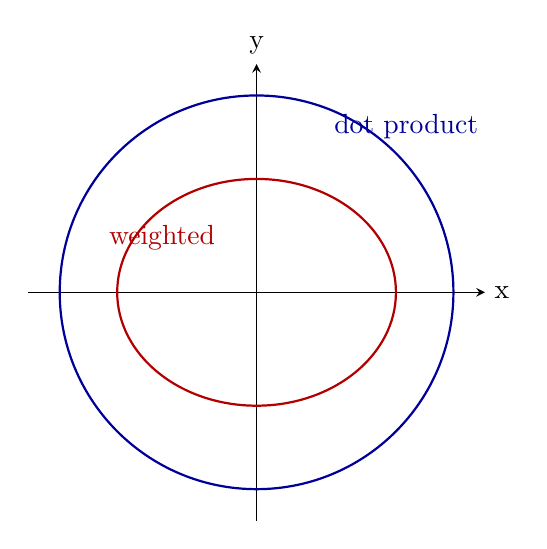
\begin{tikzpicture}[>=stealth,scale=1.0]
  \draw[->] (-2.9,0)--(2.9,0) node[right] {x};
  \draw[->] (0,-2.9)--(0,2.9) node[above] {y};
  \draw[blue!60!black,thick] (0,0) circle (2.5);
  \draw[red!70!black,thick] (0,0) ellipse (1.77 and 1.44);
  \node[blue!60!black] at (1.9,2.1) {dot product};
  \node[red!70!black] at (-1.2,0.7) {weighted};
\end{tikzpicture}
\end{center}

\noindent\textbf{Figure 1.} The vectors of length $1$ for the dot product (circle, $x^2+y^2=1$) and for the weighted inner product (ellipse, $2x^2+3y^2=1$), drawn at 2.5 cm per unit. ``Length'' and ``perpendicular'' depend on the inner product that we choose.

\begin{exmp}{Lengths and distances of polynomials}{polylen}
In $\mathbb{P}_2$ with the integral inner product, the table gives $\lVert1\rVert^2=2$, $\lVert t\rVert^2=\tfrac23$ and $\lVert t^2\rVert^2=\tfrac25$, so $\lVert1\rVert=\sqrt2$. The polynomials $1$ and $t$ are orthogonal, and so are $t$ and $t^2$, but $1$ and $t^2$ are not, since $\inner{1}{t^2}=\tfrac23$. The distance between $1$ and $t$ is
\[
\lVert1-t\rVert=\sqrt{\inner{1-t}{1-t}}=\sqrt{2+\tfrac23}=\sqrt{\tfrac83}\approx1.63 ,
\]
using $\inner{1-t}{1-t}=\inner{1}{1}-2\inner{1}{t}+\inner{t}{t}$.
\end{exmp}

\begin{exmp}{Two functions that are orthogonal}{sincos}
Let $V$ be the space of continuous functions on $[-\pi,\pi]$ with $\inner{f}{g}=\int_{-\pi}^{\pi}f(t)g(t)\,dt$. Then $\inner{\sin t}{\cos t}=\int_{-\pi}^{\pi}\sin t\cos t\,dt=\bigl[\tfrac12\sin^2t\bigr]_{-\pi}^{\pi}=0$, so $\sin t$ and $\cos t$ are orthogonal. Also $\int_{-\pi}^{\pi}\sin^2t\,dt=\pi$ and $\int_{-\pi}^{\pi}\cos^2t\,dt=\pi$. Hence $\lVert\sin t+\cos t\rVert^2=\pi+\pi=2\pi$, exactly as in the Pythagorean theorem.
\end{exmp}

\begin{thm}{Basic rules}{basic}
Let $V$ be an inner product space, $\bv{u},\bv{v},\bv{w}$ in $V$ and $c$ a scalar.
\begin{enumerate}[label=(\alph*),itemsep=1pt]
  \item $\inner{\bv{u}}{\bv{v}+\bv{w}}=\inner{\bv{u}}{\bv{v}}+\inner{\bv{u}}{\bv{w}}$ and $\inner{\bv{u}}{c\bv{v}}=c\,\inner{\bv{u}}{\bv{v}}$.
  \item $\inner{\bv{0}}{\bv{v}}=0$.
  \item $\lVert c\bv{v}\rVert=|c|\,\lVert\bv{v}\rVert$, and $\lVert\bv{v}\rVert=0$ only for $\bv{v}=\bv{0}$.
  \item $\lVert\bv{u}+\bv{v}\rVert^2=\lVert\bv{u}\rVert^2+2\inner{\bv{u}}{\bv{v}}+\lVert\bv{v}\rVert^2$ and $\lVert\bv{u}-\bv{v}\rVert^2=\lVert\bv{u}\rVert^2-2\inner{\bv{u}}{\bv{v}}+\lVert\bv{v}\rVert^2$.
  \item (Pythagorean theorem) $\bv{u}$ and $\bv{v}$ are orthogonal if and only if $\lVert\bv{u}+\bv{v}\rVert^2=\lVert\bv{u}\rVert^2+\lVert\bv{v}\rVert^2$.
\end{enumerate}
\end{thm}

\begin{proof}
(a)~By symmetry, additivity and symmetry again, $\inner{\bv{u}}{\bv{v}+\bv{w}}=\inner{\bv{v}+\bv{w}}{\bv{u}}=\inner{\bv{v}}{\bv{u}}+\inner{\bv{w}}{\bv{u}}=\inner{\bv{u}}{\bv{v}}+\inner{\bv{u}}{\bv{w}}$. The scalar rule is the same argument with homogeneity.

(b)~$\bv{0}=0\cdot\bv{0}$ (Theorem~\ref{4.1-thm:conseq}), so by homogeneity $\inner{\bv{0}}{\bv{v}}=0\cdot\inner{\bv{0}}{\bv{v}}=0$.

(c)~By (a) and rule (3), $\inner{c\bv{v}}{c\bv{v}}=c^2\inner{\bv{v}}{\bv{v}}$, and $\sqrt{c^2}=|c|$. The second claim is rule (4).

(d)~By additivity in both slots and symmetry, $\inner{\bv{u}+\bv{v}}{\bv{u}+\bv{v}}=\inner{\bv{u}}{\bv{u}}+\inner{\bv{u}}{\bv{v}}+\inner{\bv{v}}{\bv{u}}+\inner{\bv{v}}{\bv{v}}$, which is the first formula. The second is the same with $\bv{v}$ replaced by $-\bv{v}$, using (a).

(e)~By (d), $\lVert\bv{u}+\bv{v}\rVert^2-\lVert\bv{u}\rVert^2-\lVert\bv{v}\rVert^2=2\inner{\bv{u}}{\bv{v}}$, which is $0$ exactly when $\bv{u}$ and $\bv{v}$ are orthogonal.
\end{proof}

\begin{thm}{The Cauchy--Schwarz and triangle inequalities}{csip}
For all vectors $\bv{u}$ and $\bv{v}$ in an inner product space:
\begin{enumerate}[label=(\alph*),itemsep=1pt]
  \item $|\inner{\bv{u}}{\bv{v}}|\le\lVert\bv{u}\rVert\,\lVert\bv{v}\rVert$;
  \item $\lVert\bv{u}+\bv{v}\rVert\le\lVert\bv{u}\rVert+\lVert\bv{v}\rVert$.
\end{enumerate}
\end{thm}

\begin{proof}
(a)~If $\bv{v}=\bv{0}$ both sides are $0$ (Theorem~\ref{thm:basic}(b)). Otherwise let $t=\inner{\bv{u}}{\bv{v}}/\inner{\bv{v}}{\bv{v}}$. By rule (4) and Theorem~\ref{thm:basic}(d),
\[
0\le\lVert\bv{u}-t\bv{v}\rVert^2=\inner{\bv{u}}{\bv{u}}-2t\,\inner{\bv{u}}{\bv{v}}+t^2\,\inner{\bv{v}}{\bv{v}}=\lVert\bv{u}\rVert^2-\frac{\inner{\bv{u}}{\bv{v}}^2}{\lVert\bv{v}\rVert^2}.
\]
Hence $\inner{\bv{u}}{\bv{v}}^2\le\lVert\bv{u}\rVert^2\lVert\bv{v}\rVert^2$, and taking square roots gives (a).

(b)~By Theorem~\ref{thm:basic}(d) and part (a), $\lVert\bv{u}+\bv{v}\rVert^2=\lVert\bv{u}\rVert^2+2\inner{\bv{u}}{\bv{v}}+\lVert\bv{v}\rVert^2\le\lVert\bv{u}\rVert^2+2\lVert\bv{u}\rVert\lVert\bv{v}\rVert+\lVert\bv{v}\rVert^2=\bigl(\lVert\bv{u}\rVert+\lVert\bv{v}\rVert\bigr)^2$. Taking square roots of the two nonnegative sides gives (b).
\end{proof}

Part (a) is what makes the ``angle'' $\cos\theta=\inner{\bv{u}}{\bv{v}}/(\lVert\bv{u}\rVert\lVert\bv{v}\rVert)$ meaningful in every inner product space: the fraction lies between $-1$ and $1$.

\begin{exmp}{Checking the inequalities for functions}{csfun}
In $\mathbb{P}_2$ with the integral inner product take $\bv{u}=1$ and $\bv{v}=t^2$. Then $\inner{\bv{u}}{\bv{v}}=\tfrac23$, $\lVert\bv{u}\rVert^2=2$ and $\lVert\bv{v}\rVert^2=\tfrac25$. Cauchy--Schwarz says $\tfrac49\le2\cdot\tfrac25=\tfrac45$, which is true. For the triangle inequality, $\lVert1+t^2\rVert^2=2+2\cdot\tfrac23+\tfrac25=\tfrac{56}{15}$, so $\lVert1+t^2\rVert\approx1.93$, while $\lVert1\rVert+\lVert t^2\rVert\approx1.41+0.63=2.05$.
\end{exmp}

\begin{think}{Where were the coordinates?}{coords}
Look at the proof of Theorem~\ref{thm:csip}(a). Does any step use a coordinate of $\bv{u}$ or $\bv{v}$, or the fact that they are columns of numbers? What does that tell you about the inequality for polynomials and functions?
\end{think}

\begin{think}{Orthogonal for whom?}{orthwho}
The vectors $(1,2)$ and $(3,-1)$ have dot product $1$ and weighted inner product $0$ (Example~\ref{ex:weighted}). Which of the two statements ``they are orthogonal'' and ``they are at a right angle in the picture of the plane'' is true? What does the answer say about the word \emph{orthogonal}?
\end{think}

\begin{remark}[What carries over from Sections 6.1 to 6.4]
 Replace $\bv{u}\cdot\bv{v}$ by $\inner{\bv{u}}{\bv{v}}$ in each of the following proofs and read them again: the Pythagorean theorem (Theorem~\ref{6.1-thm:pyth}, now Theorem~\ref{thm:basic}(e)); the Cauchy--Schwarz and triangle inequalities (Theorem~\ref{6.1-thm:cs}, proved above); orthogonal sets are independent and the weights in an orthogonal basis (Theorems~\ref{6.2-thm:indep} and \ref{6.2-thm:weights}, below); the Best Approximation Theorem (Theorem~\ref{6.3-thm:best}); and the Gram--Schmidt process (Theorem~\ref{6.4-thm:gs}). They hold \emph{word for word}, because they use only the four rules. What does \emph{not} carry over is anything written in coordinates: the formula ``sum of products of entries'', the matrix $A\T A$, and orthogonal matrices with $Q\T Q=I$. Those belong to $\R^n$ with the dot product.
\end{remark}

% ---------------------------------------------------------------------
\subsection*{Orthogonal bases and Gram--Schmidt}

\begin{thm}{Orthogonal sets and their weights}{orthip}
Let $\bv{v}_1,\dots,\bv{v}_p$ be nonzero vectors in an inner product space, orthogonal to one another.
\begin{enumerate}[label=(\alph*),itemsep=1pt]
  \item They are linearly independent.
  \item If $\bv{y}=c_1\bv{v}_1+\cdots+c_p\bv{v}_p$, then $c_j=\dfrac{\inner{\bv{y}}{\bv{v}_j}}{\inner{\bv{v}_j}{\bv{v}_j}}$ for each $j$.
\end{enumerate}
\end{thm}

\begin{proof}
Suppose $\bv{y}=c_1\bv{v}_1+\cdots+c_p\bv{v}_p$ (for (a) take $\bv{y}=\bv{0}$). Take the inner product with $\bv{v}_j$ and use Theorem~\ref{thm:basic}(a) and orthogonality:
\[
\inner{\bv{y}}{\bv{v}_j}=c_1\inner{\bv{v}_1}{\bv{v}_j}+\cdots+c_p\inner{\bv{v}_p}{\bv{v}_j}=c_j\inner{\bv{v}_j}{\bv{v}_j}.
\]
Because $\bv{v}_j\neq\bv{0}$, $\inner{\bv{v}_j}{\bv{v}_j}>0$ by rule (4), and we may divide, which proves (b). If $\bv{y}=\bv{0}$, then $\inner{\bv{y}}{\bv{v}_j}=0$ by Theorem~\ref{thm:basic}(b), so every $c_j=0$, which is (a).
\end{proof}

\begin{exmp}{An orthogonal basis of $\mathbb{P}_2$ and weights}{polyweights}
With the integral inner product, the polynomials $1$, $t$ and $t^2-\tfrac13$ are orthogonal: $\inner{1}{t}=0$, $\inner{t}{t^2-\tfrac13}=0-0=0$ and $\inner{1}{t^2-\tfrac13}=\tfrac23-\tfrac13\cdot2=0$. Their squared lengths are $2$, $\tfrac23$ and $\lVert t^2-\tfrac13\rVert^2=\tfrac25-\tfrac29=\tfrac8{45}$. Write $p=2-t+t^2$ in this basis with Theorem~\ref{thm:orthip}(b). First $\inner{p}{1}=4+0+\tfrac23=\tfrac{14}3$, so the weight of $1$ is $\tfrac{14}{3}\big/2=\tfrac73$. Next $\inner{p}{t}=0-\tfrac23+0=-\tfrac23$, so the weight of $t$ is $-1$. Finally $\inner{p}{t^2-\tfrac13}=\inner{t^2}{t^2-\tfrac13}=\tfrac8{45}$, so the weight is $1$. Check: $\tfrac73-t+(t^2-\tfrac13)=2-t+t^2$. \ $\checkmark$
\end{exmp}

\begin{thm}{The Gram--Schmidt Process in an inner product space}{gsip}
Let $\bv{x}_1,\dots,\bv{x}_p$ be linearly independent vectors in an inner product space. Define
\[
\bv{v}_1=\bv{x}_1,\qquad \bv{v}_k=\bv{x}_k-\frac{\inner{\bv{x}_k}{\bv{v}_1}}{\inner{\bv{v}_1}{\bv{v}_1}}\bv{v}_1-\cdots-\frac{\inner{\bv{x}_k}{\bv{v}_{k-1}}}{\inner{\bv{v}_{k-1}}{\bv{v}_{k-1}}}\bv{v}_{k-1}\qquad(k=2,\dots,p).
\]
Then for every $k$ from $1$ to $p$: (a) $\bv{v}_1,\dots,\bv{v}_k$ are nonzero and orthogonal to one another; (b) $\Span\{\bv{v}_1,\dots,\bv{v}_k\}=\Span\{\bv{x}_1,\dots,\bv{x}_k\}$. So $\bv{v}_1,\dots,\bv{v}_p$ is an orthogonal basis of $\Span\{\bv{x}_1,\dots,\bv{x}_p\}$.
\end{thm}

\begin{proof}
Induction on $k$. For $k=1$, $\bv{v}_1=\bv{x}_1$ is nonzero because an independent set has no zero vector, and (b) is trivial.

Let $k\ge2$ and assume (a) and (b) for $k-1$. For $j<k$, take the inner product of the definition of $\bv{v}_k$ with $\bv{v}_j$. All terms $\inner{\bv{v}_i}{\bv{v}_j}$ with $i\neq j$ are $0$ by assumption, so
\[
\inner{\bv{v}_k}{\bv{v}_j}=\inner{\bv{x}_k}{\bv{v}_j}-\frac{\inner{\bv{x}_k}{\bv{v}_j}}{\inner{\bv{v}_j}{\bv{v}_j}}\inner{\bv{v}_j}{\bv{v}_j}=0 .
\]
If $\bv{v}_k$ were $\bv{0}$, then $\bv{x}_k$ would be a combination of $\bv{v}_1,\dots,\bv{v}_{k-1}$, hence of $\bv{x}_1,\dots,\bv{x}_{k-1}$ by (b), and $\bv{x}_1,\dots,\bv{x}_k$ would be dependent. So $\bv{v}_k\neq\bv{0}$, and (a) holds. For (b): $\bv{v}_k$ is $\bv{x}_k$ minus a combination of $\bv{v}_1,\dots,\bv{v}_{k-1}$, which lie in $\Span\{\bv{x}_1,\dots,\bv{x}_{k-1}\}$; so $\Span\{\bv{v}_1,\dots,\bv{v}_k\}\subseteq\Span\{\bv{x}_1,\dots,\bv{x}_k\}$. Conversely $\bv{x}_k=\bv{v}_k+(\text{a combination of }\bv{v}_1,\dots,\bv{v}_{k-1})$, and $\bv{x}_1,\dots,\bv{x}_{k-1}$ are in $\Span\{\bv{v}_1,\dots,\bv{v}_{k-1}\}$ by assumption. The spans are equal. The orthogonal vectors are independent by Theorem~\ref{thm:orthip}(a), so they form a basis.
\end{proof}

The procedure is exactly Procedure~\ref{6.4-proc:gsproc}, with every dot product replaced by $\inner{\cdot}{\cdot}$.

\begin{exmp}{Gram--Schmidt on $1,t,t^2$ for the integral}{gsint}
The polynomials $\bv{x}_1=1$, $\bv{x}_2=t$, $\bv{x}_3=t^2$ are independent, since $a+bt+ct^2$ is the zero polynomial only when $a=b=c=0$. Take $\bv{v}_1=1$ with $\inner{\bv{v}_1}{\bv{v}_1}=2$. Since $\inner{t}{1}=0$, $\bv{v}_2=t$, with $\inner{\bv{v}_2}{\bv{v}_2}=\tfrac23$. For $\bv{x}_3$ we need $\inner{t^2}{1}=\tfrac23$ and $\inner{t^2}{t}=0$:
\[
\bv{v}_3=t^2-\frac{2/3}{2}\cdot1-\frac{0}{2/3}\,t=t^2-\tfrac13 .
\]
This is the basis used in Example~\ref{ex:polyweights}, with $\lVert\bv{v}_3\rVert^2=\tfrac8{45}$.
\end{exmp}

\begin{exmp}{The same polynomials for the three-point inner product}{gsev}
Use the inner product of Example~\ref{ex:evalip} and the same $\bv{x}_1=1$, $\bv{x}_2=t$, $\bv{x}_3=t^2$. The values at $-1,0,1$ are $(1,1,1)$, $(-1,0,1)$ and $(1,0,1)$, so $\inner{1}{1}=3$, $\inner{t}{1}=0$, $\inner{t}{t}=2$, $\inner{t^2}{1}=2$ and $\inner{t^2}{t}=0$. Hence $\bv{v}_1=1$, $\bv{v}_2=t$ and
\[
\bv{v}_3=t^2-\tfrac23\cdot1-\tfrac02\,t=t^2-\tfrac23 ,
\]
with values $(\tfrac13,-\tfrac23,\tfrac13)$ at $-1,0,1$. Taking $3\bv{v}_3=3t^2-2$, with values $(1,-2,1)$, we get $\inner{3t^2-2}{3t^2-2}=6$. The first two vectors are the same as for the integral, the third is not: a different inner product gives a different orthogonal basis of the same space.
\end{exmp}

\begin{think}{Does the zero vector appear?}{gsdep}
In the proof of Theorem~\ref{thm:gsip}, where is independence of $\bv{x}_1,\dots,\bv{x}_p$ used? What happens in the process if $\bv{x}_3$ is a combination of $\bv{x}_1$ and $\bv{x}_2$?
\end{think}

\begin{kc}{One Gram--Schmidt step}{kcgs}
In $\mathbb{P}_2$ with the integral inner product, apply the process to $\bv{x}_1=1+t$ and $\bv{x}_2=1-t$. First compute $\inner{1+t}{1+t}$ and $\inner{1-t}{1+t}$, then $\bv{v}_2$. Check that $\inner{\bv{v}_1}{\bv{v}_2}=0$.
\end{kc}

% ---------------------------------------------------------------------
\subsection*{Best approximation}

\begin{thm}{Best Approximation in an inner product space}{bestip}
Let $W$ be a subspace of an inner product space $V$ with an orthogonal basis $\bv{v}_1,\dots,\bv{v}_p$ (nonzero, orthogonal to one another). For $\bv{y}$ in $V$ put
\[
\hat{\bv{y}}=\frac{\inner{\bv{y}}{\bv{v}_1}}{\inner{\bv{v}_1}{\bv{v}_1}}\bv{v}_1+\cdots+\frac{\inner{\bv{y}}{\bv{v}_p}}{\inner{\bv{v}_p}{\bv{v}_p}}\bv{v}_p .
\]
\begin{enumerate}[label=(\alph*),itemsep=1pt]
  \item $\bv{y}-\hat{\bv{y}}$ is orthogonal to every vector of $W$.
  \item For every $\bv{w}$ in $W$ with $\bv{w}\neq\hat{\bv{y}}$: $\lVert\bv{y}-\hat{\bv{y}}\rVert<\lVert\bv{y}-\bv{w}\rVert$. So $\hat{\bv{y}}$ is the unique closest vector of $W$ to $\bv{y}$.
  \item $\lVert\bv{y}-\hat{\bv{y}}\rVert^2=\lVert\bv{y}\rVert^2-\displaystyle\sum_{j=1}^{p}\frac{\inner{\bv{y}}{\bv{v}_j}^2}{\inner{\bv{v}_j}{\bv{v}_j}}$.
\end{enumerate}
\end{thm}

\begin{proof}
(a)~By Theorem~\ref{thm:basic}(a) and orthogonality of the basis, $\inner{\hat{\bv{y}}}{\bv{v}_j}=\dfrac{\inner{\bv{y}}{\bv{v}_j}}{\inner{\bv{v}_j}{\bv{v}_j}}\inner{\bv{v}_j}{\bv{v}_j}=\inner{\bv{y}}{\bv{v}_j}$, so $\inner{\bv{y}-\hat{\bv{y}}}{\bv{v}_j}=0$ for each $j$. Every $\bv{w}$ in $W$ is a combination of the $\bv{v}_j$, so $\inner{\bv{y}-\hat{\bv{y}}}{\bv{w}}=0$.

(b)~Write $\bv{y}-\bv{w}=(\bv{y}-\hat{\bv{y}})+(\hat{\bv{y}}-\bv{w})$. The second vector is in $W$, so by (a) the two are orthogonal, and by the Pythagorean theorem (Theorem~\ref{thm:basic}(e)), $\lVert\bv{y}-\bv{w}\rVert^2=\lVert\bv{y}-\hat{\bv{y}}\rVert^2+\lVert\hat{\bv{y}}-\bv{w}\rVert^2$. If $\bv{w}\neq\hat{\bv{y}}$ the last term is positive, which gives (b).

(c)~Since $\hat{\bv{y}}$ and $\bv{y}-\hat{\bv{y}}$ are orthogonal, $\lVert\bv{y}\rVert^2=\lVert\hat{\bv{y}}\rVert^2+\lVert\bv{y}-\hat{\bv{y}}\rVert^2$. The orthogonal terms of $\hat{\bv{y}}$ give $\lVert\hat{\bv{y}}\rVert^2=\sum_j\inner{\bv{y}}{\bv{v}_j}^2/\inner{\bv{v}_j}{\bv{v}_j}$ (Theorem~\ref{thm:basic}(e) repeatedly with Theorem~\ref{thm:basic}(c)).
\end{proof}

Which subspaces have an orthogonal basis? Every subspace spanned by finitely many independent vectors, by Theorem~\ref{thm:gsip}. So $\hat{\bv{y}}=\proj_W\bv{y}$ exists whenever $W$ is of this kind, and by (b) it does not depend on which orthogonal basis was used.

\begin{proc}{Best approximation from an orthogonal basis}{bestproc}
\begin{enumerate}[nosep]
  \item Find an orthogonal basis $\bv{v}_1,\dots,\bv{v}_p$ of $W$ (Gram--Schmidt, if necessary).
  \item Compute the numbers $\inner{\bv{y}}{\bv{v}_j}$ and $\inner{\bv{v}_j}{\bv{v}_j}$.
  \item Form $\hat{\bv{y}}=\sum_j\frac{\inner{\bv{y}}{\bv{v}_j}}{\inner{\bv{v}_j}{\bv{v}_j}}\bv{v}_j$.
  \item Check that $\inner{\bv{y}-\hat{\bv{y}}}{\bv{v}_j}=0$ for every $j$.
  \item The error is $\lVert\bv{y}-\hat{\bv{y}}\rVert$, with the squared error from Theorem~\ref{thm:bestip}(c).
\end{enumerate}
\end{proc}

\begin{exmp}{The best line for $t^3$}{cubic}
In the space of continuous functions on $[-1,1]$ with $\inner{f}{g}=\int_{-1}^1f(t)g(t)\,dt$, find the polynomial of degree at most $1$ closest to $f(t)=t^3$. Here $W=\mathbb{P}_1$ has the orthogonal basis $1,t$ with $\inner{1}{1}=2$ and $\inner{t}{t}=\tfrac23$. Then $\inner{t^3}{1}=\int_{-1}^1t^3\,dt=0$ and $\inner{t^3}{t}=\int_{-1}^1t^4\,dt=\tfrac25$, so
\[
\hat{f}=\frac02\cdot1+\frac{2/5}{2/3}\,t=\tfrac35\,t .
\]
Check: $\inner{t^3-\tfrac35t}{t}=\tfrac25-\tfrac35\cdot\tfrac23=0$ and $\inner{t^3-\tfrac35t}{1}=0-0=0$. \ $\checkmark$ The squared error is $\lVert t^3\rVert^2-\lVert\hat f\rVert^2=\tfrac27-\tfrac9{25}\cdot\tfrac23=\tfrac27-\tfrac6{25}=\tfrac8{175}$.
\end{exmp}

\begin{center}
\begin{tikzpicture}[>=stealth,scale=1.0]
  \draw[->] (-2.9,0)--(2.9,0) node[right] {t};
  \draw[->] (0,-2.9)--(0,2.9) node[above] {y};
  \draw[blue!60!black,thick,domain=-1:1,samples=41,smooth] plot (\x*2.5,\x*\x*\x*2.5);
  \draw[red!70!black,thick] (-2.5,-1.5)--(2.5,1.5);
  \node[blue!60!black] at (1.9,2.5) {t cubed};
  \node[red!70!black] at (2.2,0.7) {0.6 t};
\end{tikzpicture}
\end{center}

\noindent\textbf{Figure 2.} The function $t^3$ and its best approximation $\tfrac35t$ on $[-1,1]$ (2.5 cm per unit on both axes). The line is not the closest line at any single point; it is closest in the sense of the integral of the squared gap.

\begin{exmp}{A quadratic approximation of $|t|$}{abs}
Let $V$ be the continuous functions on $[-1,1]$ with the integral inner product, and $f(t)=|t|$, which is not a polynomial. The subspace $W=\mathbb{P}_2$ has the orthogonal basis $1,\ t,\ t^2-\tfrac13$ of Example~\ref{ex:gsint}. Splitting the integrals at $0$: $\inner{|t|}{1}=2\int_0^1t\,dt=1$, $\inner{|t|}{t}=0$ (the integrand is odd) and
\[
\inner{|t|}{t^2-\tfrac13}=2\int_0^1\bigl(t^3-\tfrac13t\bigr)\,dt=2\bigl(\tfrac14-\tfrac16\bigr)=\tfrac16 .
\]
The weights are $\tfrac12$, $0$ and $\tfrac{1/6}{8/45}=\tfrac{15}{16}$, so
\[
\hat f=\tfrac12+\tfrac{15}{16}\bigl(t^2-\tfrac13\bigr)=\tfrac3{16}+\tfrac{15}{16}t^2 .
\]
The squared error is $\lVert|t|\rVert^2-\bigl(\tfrac{1^2}{2}+\tfrac{(1/6)^2}{8/45}\bigr)=\tfrac23-\tfrac12-\tfrac5{32}=\tfrac1{96}$, using $\int_{-1}^1t^2\,dt=\tfrac23$. The error $\lVert f-\hat f\rVert=\sqrt{1/96}\approx0.10$ is small next to $\lVert f\rVert=\sqrt{2/3}\approx0.82$.
\end{exmp}

\begin{think}{Best for whom?}{bestwho}
Find the constant closest to $t^2$ in $\mathbb{P}_2$ for the integral inner product, and then for the three-point inner product of Example~\ref{ex:evalip}. Why are the answers different?
\end{think}

\begin{kc}{Best constant}{kcconst}
For the integral inner product on $[-1,1]$, find the multiple of $1$ closest to $t^2$, and the squared error.
\end{kc}

\begin{kc}{True or false?}{kctf}
Give a reason. (a)~Every inner product on $\R^2$ is the dot product. (b)~The Cauchy--Schwarz inequality holds in every inner product space. (c)~If $\inner{\bv{u}}{\bv{v}}=0$, the arrows $\bv{u}$ and $\bv{v}$ meet at a right angle. (d)~If $\inner{\bv{v}}{\bv{v}}=0$, then $\bv{v}=\bv{0}$.
\end{kc}

% ---------------------------------------------------------------------
\subsection*{Summary}
\begin{itemize}
  \item \textbf{Inner product.} A rule with symmetry, additivity, homogeneity and positive definiteness (Definition~\ref{def:ip}). Examples: weighted dot products, $\int_a^bf g\,dt$ on functions, sums of values at points (but only where no nonzero vector has length $0$).
  \item \textbf{Geometry.} Length, distance and orthogonality are defined from $\inner{\cdot}{\cdot}$ (Definition~\ref{def:lenip}) and depend on the inner product. The Pythagorean theorem, Cauchy--Schwarz and the triangle inequality hold (Theorems~\ref{thm:basic} and \ref{thm:csip}).
  \item \textbf{Orthogonal bases.} Orthogonal sets are independent and give weights $\inner{\bv{y}}{\bv{v}_j}/\inner{\bv{v}_j}{\bv{v}_j}$ (Theorem~\ref{thm:orthip}). Gram--Schmidt produces them (Theorem~\ref{thm:gsip}).
  \item \textbf{Best approximation.} $\hat{\bv{y}}=\sum_j\frac{\inner{\bv{y}}{\bv{v}_j}}{\inner{\bv{v}_j}{\bv{v}_j}}\bv{v}_j$ is the unique closest vector of $W$ to $\bv{y}$ and the error is $\lVert\bv{y}-\hat{\bv{y}}\rVert$ (Theorem~\ref{thm:bestip}). For functions this is approximation in the mean-square sense.
\end{itemize}

\subsection*{Questions to think about before the next section}
\begin{enumerate}[nosep]
  \item Which formulas in this section would stop making sense if we dropped rule (4)?
  \item Two inner products on the same space can disagree about which vectors are orthogonal. Is there any inner product for which $1$ and $t^2$ are orthogonal in $\mathbb{P}_2$?
  \item The best approximation of $t^3$ by a line was $\tfrac35t$, no matter which of the two orthogonal bases $\{1,t\}$ or $\{3,2t\}$ we use. Why?
\end{enumerate}

% ---------------------------------------------------------------------
\subsection*{Example bank}
The twelve examples below add problem types that the worked examples above do not cover: checking the rules for a non-diagonal inner product and for rules that fail; lengths and angles of polynomials, the inequalities for functions on $[0,1]$, and orthogonal functions; Gram--Schmidt in a weighted $\R^3$ and one more step in $\mathbb{P}_3$; best linear approximations of $t^2$ and $t^3$ on $[0,1]$; and three proofs. Within each group the examples go from easier to harder. Work each problem before you read its solution.

\textbf{What is in this bank.}
\begin{itemize}
  \item \textbf{Bank A, checking the rules:} Example~\ref{ex:b-check} (a non-diagonal inner product on $\R^2$) and Example~\ref{ex:b-notip} (two rules that fail).
  \item \textbf{Bank B, lengths and inequalities:} Example~\ref{ex:b-ipnum} (an angle between polynomials), Example~\ref{ex:b-csnum} (the inequalities on $[0,1]$) and Example~\ref{ex:b-pyth} (orthogonal functions).
  \item \textbf{Bank C, Gram--Schmidt:} Example~\ref{ex:b-gsw} (weighted $\R^3$) and Example~\ref{ex:b-gsint} (the next polynomial).
  \item \textbf{Bank D, best approximation:} Example~\ref{ex:b-best1} (a line for $t^2$ on $[0,1]$) and Example~\ref{ex:b-best2} (a line for $t^3$ on $[0,1]$).
  \item \textbf{Bank E, proofs:} Example~\ref{ex:b-pos} (beginner: $\inner{\bv{u}}{\bv{w}}=0$ for all $\bv{w}$), Example~\ref{ex:b-par} (intermediate: the parallelogram law) and Example~\ref{ex:b-equal} (intermediate: equality in Cauchy--Schwarz).
\end{itemize}

\subsection*{Bank A: Checking the rules}
\begin{exmp}{A non-diagonal inner product}{b-check}
Show that $\inner{\bv{u}}{\bv{v}}=u_1v_1+u_1v_2+u_2v_1+2u_2v_2$ is an inner product on $\R^2$, and find a vector orthogonal to $(1,0)$.

\textbf{Solution.} Swapping $\bv{u}$ and $\bv{v}$ gives the same four terms, so (1) holds. Each term is a constant times one coordinate of $\bv{u}$ times one coordinate of $\bv{v}$, so the rule respects sums and scalars in $\bv{u}$: (2) and (3). For (4), complete the square: $\inner{\bv{u}}{\bv{u}}=u_1^2+2u_1u_2+2u_2^2=(u_1+u_2)^2+u_2^2\ge0$, and it is $0$ only if $u_2=0$ and $u_1+u_2=0$, that is $\bv{u}=\bv{0}$. For the orthogonal vector, $\inner{(1,0)}{(v_1,v_2)}=v_1+v_2$, so any $\bv{v}$ with $v_1=-v_2$ works, for example $(1,-1)$. Check: $\inner{(1,0)}{(1,-1)}=1-1+0+0=0$, while the dot product is $1$. The vector $(1,-1)$ has $\inner{(1,-1)}{(1,-1)}=1-2+2=1$, so it is a unit vector for this inner product.
\end{exmp}

\begin{exmp}{Two rules that are not inner products}{b-notip}
Why is each rule not an inner product? (a)~On $\mathbb{P}_2$, $\inner{p}{q}=p(0)q(0)+p(1)q(1)$. (b)~On $\R^2$, $\inner{\bv{u}}{\bv{v}}=u_1v_2+u_2v_1$.

\textbf{Solution.} (a)~Take $p(t)=t^2-t$, which is not the zero polynomial. Then $p(0)=0$ and $p(1)=0$, so $\inner{p}{p}=0$, and the second part of rule (4) fails. Two values cannot detect a polynomial of degree $2$; on $\mathbb{P}_1$ the same rule is an inner product, since two values determine $a+bt$. (b)~Rules (1) to (3) hold, but $\inner{(1,-1)}{(1,-1)}=1\cdot(-1)+(-1)\cdot1=-2<0$, so the first part of rule (4) fails.
\end{exmp}

\subsection*{Bank B: Lengths and inequalities}
\begin{exmp}{An angle between polynomials}{b-ipnum}
In $\mathbb{P}_2$ with $\inner{p}{q}=\int_{-1}^1p(t)q(t)\,dt$, find the angle between $p=t+t^2$ and $q=1-t^2$.

\textbf{Solution.} $\inner{p}{q}=\int_{-1}^1(t+t^2-t^3-t^4)\,dt=0+\tfrac23-0-\tfrac25=\tfrac4{15}$. Also $\lVert p\rVert^2=\int_{-1}^1(t^2+2t^3+t^4)\,dt=\tfrac23+0+\tfrac25=\tfrac{16}{15}$ and $\lVert q\rVert^2=\int_{-1}^1(1-2t^2+t^4)\,dt=2-\tfrac43+\tfrac25=\tfrac{16}{15}$. So $\cos\theta=\dfrac{4/15}{16/15}=\tfrac14$ and $\theta\approx75.5^\circ$. The fraction is between $-1$ and $1$, as Theorem~\ref{thm:csip}(a) promises.
\end{exmp}

\begin{exmp}{The inequalities on $[0,1]$}{b-csnum}
On the continuous functions on $[0,1]$ with $\inner{f}{g}=\int_0^1f(t)g(t)\,dt$, check Cauchy--Schwarz and the triangle inequality for $f=t$ and $g=t^2$.

\textbf{Solution.} $\inner{f}{g}=\int_0^1t^3\,dt=\tfrac14$, $\lVert f\rVert^2=\int_0^1t^2\,dt=\tfrac13$ and $\lVert g\rVert^2=\int_0^1t^4\,dt=\tfrac15$. Cauchy--Schwarz in squared form: $\bigl(\tfrac14\bigr)^2=\tfrac1{16}\le\tfrac13\cdot\tfrac15=\tfrac1{15}$, true, and close because $t$ and $t^2$ are nearly parallel as functions on $[0,1]$. For the triangle inequality, $\lVert f+g\rVert^2=\tfrac13+2\cdot\tfrac14+\tfrac15=\tfrac{31}{30}\approx1.033$, so $\lVert f+g\rVert\approx1.017$, and $\lVert f\rVert+\lVert g\rVert\approx0.577+0.447=1.025$.
\end{exmp}

\begin{exmp}{Orthogonal functions and the Pythagorean theorem}{b-pyth}
In the functions on $[-\pi,\pi]$ with $\inner{f}{g}=\int_{-\pi}^{\pi}fg\,dt$, find $\lVert\sin t+2\cos t\rVert$. Are $t$ and $\sin t$ orthogonal?

\textbf{Solution.} By Example~\ref{ex:sincos}, $\sin t\perp\cos t$ and $\lVert\sin t\rVert^2=\lVert\cos t\rVert^2=\pi$. By Theorem~\ref{thm:basic}(c) $\lVert2\cos t\rVert^2=4\pi$, and by the Pythagorean theorem $\lVert\sin t+2\cos t\rVert^2=\pi+4\pi=5\pi$, so the length is $\sqrt{5\pi}$. For the second question, integrate by parts: $\int_{-\pi}^{\pi}t\sin t\,dt=\bigl[-t\cos t+\sin t\bigr]_{-\pi}^{\pi}=\pi+\pi=2\pi\neq0$. So $t$ and $\sin t$ are not orthogonal.
\end{exmp}

\subsection*{Bank C: Gram--Schmidt}
\begin{exmp}{Gram--Schmidt in a weighted $\R^3$}{b-gsw}
On $\R^3$ let $\inner{\bv{u}}{\bv{v}}=u_1v_1+2u_2v_2+3u_3v_3$. Apply the process to $\bv{x}_1=(1,1,1)$, $\bv{x}_2=(1,0,-1)$ and $\bv{x}_3=(0,1,0)$.

\textbf{Solution.} Take $\bv{v}_1=\bv{x}_1$, with $\inner{\bv{v}_1}{\bv{v}_1}=1+2+3=6$. Then $\inner{\bv{x}_2}{\bv{v}_1}=1+0-3=-2$, so $\bv{v}_2=\bv{x}_2+\tfrac13\bv{v}_1=(\tfrac43,\tfrac13,-\tfrac23)=\tfrac13(4,1,-2)$. Take $\bv{v}_2=(4,1,-2)$, with $\inner{\bv{v}_2}{\bv{v}_2}=16+2+12=30$. Next $\inner{\bv{x}_3}{\bv{v}_1}=2$ and $\inner{\bv{x}_3}{\bv{v}_2}=2$, so
\[
\bv{v}_3=\bv{x}_3-\tfrac26\bv{v}_1-\tfrac2{30}\bv{v}_2=(0,1,0)-(\tfrac13,\tfrac13,\tfrac13)-(\tfrac4{15},\tfrac1{15},-\tfrac2{15})=(-\tfrac35,\tfrac35,-\tfrac15)=\tfrac15(-3,3,-1).
\]
Take $\bv{v}_3=(-3,3,-1)$, with $\inner{\bv{v}_3}{\bv{v}_3}=9+18+3=30$. Check: $\inner{\bv{v}_1}{\bv{v}_2}=4+2-6=0$, $\inner{\bv{v}_1}{\bv{v}_3}=-3+6-3=0$ and $\inner{\bv{v}_2}{\bv{v}_3}=-12+6+6=0$. \ $\checkmark$ Notice that the dot products of these vectors are not $0$ (for instance $(4,1,-2)\cdot(-3,3,-1)=-7$): orthogonality refers to the weighted rule.
\end{exmp}

\begin{exmp}{The next polynomial}{b-gsint}
In $\mathbb{P}_3$ with the integral inner product on $[-1,1]$, continue Example~\ref{ex:gsint} with $\bv{x}_4=t^3$.

\textbf{Solution.} The vectors $\bv{v}_1=1$, $\bv{v}_2=t$ and $\bv{v}_3=t^2-\tfrac13$ are already orthogonal. Because $t^3$ is odd, $\inner{t^3}{1}=0$ and $\inner{t^3}{t^2-\tfrac13}=0$, and $\inner{t^3}{t}=\tfrac25$. So $\bv{v}_4=t^3-\tfrac{2/5}{2/3}\,t=t^3-\tfrac35t$, with $\lVert\bv{v}_4\rVert^2=\tfrac27-\tfrac6{25}=\tfrac8{175}$. This is the error of Example~\ref{ex:cubic}: by Theorem~\ref{thm:bestip}, $\bv{v}_4$ is the part of $t^3$ that is orthogonal to $\mathbb{P}_2$.
\end{exmp}

\subsection*{Bank D: Best approximation}
\begin{exmp}{A line for $t^2$ on $[0,1]$}{b-best1}
On the continuous functions on $[0,1]$ with $\inner{f}{g}=\int_0^1fg\,dt$, find the polynomial of degree at most $1$ closest to $f=t^2$.

\textbf{Solution.} The polynomials $1$ and $t-\tfrac12$ are orthogonal: $\inner{1}{t-\tfrac12}=\tfrac12-\tfrac12=0$. They have $\inner{1}{1}=1$ and $\lVert t-\tfrac12\rVert^2=\int_0^1(t^2-t+\tfrac14)\,dt=\tfrac13-\tfrac12+\tfrac14=\tfrac1{12}$. Then $\inner{t^2}{1}=\tfrac13$ and $\inner{t^2}{t-\tfrac12}=\tfrac14-\tfrac16=\tfrac1{12}$, so the weights are $\tfrac13$ and $1$ and
\[
\hat f=\tfrac13+\bigl(t-\tfrac12\bigr)=t-\tfrac16 .
\]
The squared error is $\lVert t^2\rVert^2-\bigl(\tfrac{(1/3)^2}{1}+\tfrac{(1/12)^2}{1/12}\bigr)=\tfrac15-\tfrac19-\tfrac1{12}=\tfrac1{180}$.
\end{exmp}

\begin{exmp}{A line for $t^3$ on $[0,1]$}{b-best2}
In the same space, find the polynomial of degree at most $1$ closest to $f=t^3$, and verify that the residual is orthogonal to $1$ and to $t$.

\textbf{Solution.} With the orthogonal basis $1,\ t-\tfrac12$ of the previous example: $\inner{t^3}{1}=\tfrac14$ and $\inner{t^3}{t-\tfrac12}=\tfrac15-\tfrac18=\tfrac3{40}$. The weights are $\tfrac14$ and $\tfrac{3/40}{1/12}=\tfrac9{10}$, so $\hat f=\tfrac14+\tfrac9{10}\bigl(t-\tfrac12\bigr)=\tfrac9{10}t-\tfrac15$. Residual $r=t^3-\tfrac9{10}t+\tfrac15$: $\inner{r}{1}=\tfrac14-\tfrac9{20}+\tfrac15=0$ and $\inner{r}{t}=\tfrac15-\tfrac9{10}\cdot\tfrac13+\tfrac15\cdot\tfrac12=\tfrac15-\tfrac3{10}+\tfrac1{10}=0$. \ $\checkmark$ The squared error is $\tfrac17-\tfrac1{16}-\tfrac{(3/40)^2}{1/12}=\tfrac17-\tfrac1{16}-\tfrac{27}{400}=\tfrac9{700}$.
\end{exmp}

\subsection*{Bank E: Proofs}
\begin{exmp}{Orthogonal to everything}{b-pos}
\textbf{Statement.} If $\inner{\bv{u}}{\bv{w}}=0$ for every $\bv{w}$ in $V$, then $\bv{u}=\bv{0}$.

\textbf{Plan.} We may choose $\bv{w}$ as we like, so choose the vector that makes rule (4) applicable.

\textbf{Proof.}
\emph{Step 1 (choose $\bv{w}=\bv{u}$).} The hypothesis holds for every vector, in particular for $\bv{w}=\bv{u}$, so $\inner{\bv{u}}{\bv{u}}=0$.
\emph{Step 2 (use rule (4)).} By the second part of rule (4), $\inner{\bv{u}}{\bv{u}}=0$ forces $\bv{u}=\bv{0}$. \qquad$\blacksquare$

\textbf{Common mistake.} Using only one $\bv{w}$ that you happen to have in front of you. In Example~\ref{ex:weighted}, $\bv{u}=(1,2)$ has $\inner{\bv{u}}{\bv{w}}=0$ for $\bv{w}=(3,-1)$, and $\bv{u}\neq\bv{0}$. The hypothesis must hold for \emph{all} $\bv{w}$, and Step~1 uses exactly that.
\end{exmp}

\begin{exmp}{The parallelogram law}{b-par}
\textbf{Statement.} For all $\bv{u},\bv{v}$ in an inner product space, $\lVert\bv{u}+\bv{v}\rVert^2+\lVert\bv{u}-\bv{v}\rVert^2=2\lVert\bv{u}\rVert^2+2\lVert\bv{v}\rVert^2$.

\textbf{Plan.} Expand both squared lengths with Theorem~\ref{thm:basic}(d) and add.

\textbf{Proof.}
\emph{Step 1 (expand the sum).} $\lVert\bv{u}+\bv{v}\rVert^2=\lVert\bv{u}\rVert^2+2\inner{\bv{u}}{\bv{v}}+\lVert\bv{v}\rVert^2$.
\emph{Step 2 (expand the difference).} $\lVert\bv{u}-\bv{v}\rVert^2=\lVert\bv{u}\rVert^2-2\inner{\bv{u}}{\bv{v}}+\lVert\bv{v}\rVert^2$.
\emph{Step 3 (add).} The terms $\pm2\inner{\bv{u}}{\bv{v}}$ cancel and what remains is $2\lVert\bv{u}\rVert^2+2\lVert\bv{v}\rVert^2$. \qquad$\blacksquare$

\textbf{Common mistake.} Dropping the cross term in only one of the two expansions, or believing that $\lVert\bv{u}+\bv{v}\rVert^2=\lVert\bv{u}\rVert^2+\lVert\bv{v}\rVert^2$ always; that holds only for orthogonal vectors. Numerical check with Example~\ref{ex:weighted}, $\bv{u}=(1,2)$ and $\bv{v}=(3,-1)$: $\bv{u}+\bv{v}=(4,1)$ has squared length $32+3=35$, $\bv{u}-\bv{v}=(-2,3)$ has squared length $8+27=35$, and $35+35=70=2\cdot14+2\cdot21$. In $\mathbb{P}_2$ with the integral: $\lVert1+t\rVert^2=\lVert1-t\rVert^2=\tfrac83$ and $\tfrac83+\tfrac83=\tfrac{16}3=2\cdot2+2\cdot\tfrac23$.
\end{exmp}

\begin{exmp}{When is Cauchy--Schwarz an equality?}{b-equal}
\textbf{Statement.} If $\bv{v}\neq\bv{0}$ and $|\inner{\bv{u}}{\bv{v}}|=\lVert\bv{u}\rVert\,\lVert\bv{v}\rVert$, then $\bv{u}$ is a multiple of $\bv{v}$.

\textbf{Plan.} Reread the proof of Theorem~\ref{thm:csip}(a): the inequality came from $\lVert\bv{u}-t\bv{v}\rVert^2\ge0$. Equality should make this quantity $0$.

\textbf{Proof.}
\emph{Step 1 (the vector).} Let $t=\inner{\bv{u}}{\bv{v}}/\inner{\bv{v}}{\bv{v}}$, defined since $\bv{v}\neq\bv{0}$.
\emph{Step 2 (the identity).} From the proof of Theorem~\ref{thm:csip}(a), $\lVert\bv{u}-t\bv{v}\rVert^2=\lVert\bv{u}\rVert^2-\inner{\bv{u}}{\bv{v}}^2/\lVert\bv{v}\rVert^2$.
\emph{Step 3 (use equality).} Squaring the hypothesis gives $\inner{\bv{u}}{\bv{v}}^2=\lVert\bv{u}\rVert^2\lVert\bv{v}\rVert^2$, so the right side of Step~2 is $0$.
\emph{Step 4 (conclude).} $\lVert\bv{u}-t\bv{v}\rVert=0$ means $\bv{u}-t\bv{v}=\bv{0}$ (Theorem~\ref{thm:basic}(c)), so $\bv{u}=t\bv{v}$. \qquad$\blacksquare$

\textbf{Common mistake.} Concluding $\bv{u}=\bv{v}$; the multiple is $t$, which may be any number (and negative). Numerical check in $\mathbb{P}_2$ with the integral: $\bv{u}=3t$, $\bv{v}=t$ give $\inner{\bv{u}}{\bv{v}}=2$, $\lVert\bv{u}\rVert\lVert\bv{v}\rVert=\sqrt{6}\cdot\sqrt{2/3}=2$, and $t=2\big/\tfrac23=3$, so $\bv{u}=3\bv{v}$.
\end{exmp}

\subsection*{Answers and discussion}
\begin{description}[leftmargin=0pt,itemsep=5pt]
  \item[Knowledge Check \ref{kc:kcweight}.] $\inner{(2,1)}{(1,-2)}=2\cdot2\cdot1+3\cdot1\cdot(-2)=4-6=-2$, and $\inner{(2,1)}{(2,1)}=8+3=11$. Since $-2\neq0$, the vectors are not orthogonal for this inner product.
  \item[Knowledge Check \ref{kc:kcwhich}.] (a)~Yes: the same check as in Example~\ref{ex:weighted} with weights $1$ and $3$. (b)~No: $\inner{(1,-1)}{(1,-1)}=1-1-1+1=0$ although $(1,-1)\neq\bv{0}$; in general $\inner{\bv{u}}{\bv{u}}=(u_1+u_2)^2$. (c)~Yes: $\inner{\bv{u}}{\bv{u}}=(u_1+u_2)^2+u_2^2$, as in Example~\ref{ex:b-check}.
  \item[Knowledge Check \ref{kc:kcgs}.] $\inner{1+t}{1+t}=\int_{-1}^1(1+2t+t^2)\,dt=2+0+\tfrac23=\tfrac83$ and $\inner{1-t}{1+t}=\int_{-1}^1(1-t^2)\,dt=2-\tfrac23=\tfrac43$. Then $\bv{v}_2=(1-t)-\tfrac{4/3}{8/3}(1+t)=(1-t)-\tfrac12(1+t)=\tfrac12-\tfrac32t=\tfrac12(1-3t)$; take $\bv{v}_2=1-3t$. Check: $\inner{1+t}{1-3t}=\int_{-1}^1(1-2t-3t^2)\,dt=2-0-2=0$.
  \item[Knowledge Check \ref{kc:kcconst}.] $\inner{t^2}{1}=\tfrac23$ and $\inner{1}{1}=2$, so $\hat f=\tfrac13$. The squared error is $\lVert t^2\rVert^2-\tfrac{(2/3)^2}{2}=\tfrac25-\tfrac29=\tfrac8{45}$ (this is $\lVert t^2-\tfrac13\rVert^2$ of Example~\ref{ex:polyweights}).
  \item[Knowledge Check \ref{kc:kctf}.] (a)~False: Example~\ref{ex:weighted} is another one. (b)~True: Theorem~\ref{thm:csip}. (c)~False: orthogonality is relative to the inner product; in Example~\ref{ex:weighted} the arrows $(1,2)$ and $(3,-1)$ are orthogonal but are not at a right angle in the picture. (d)~True: rule (4).
  \item[Pause and think \ref{think:noneg}.] $\sqrt{-1}$ is not a real number, so the length would not exist. Rule (4), $\inner{\bv{u}}{\bv{u}}\ge0$, guarantees that the square root in Definition~\ref{def:lenip} is defined; its second part guarantees that only the zero vector has length $0$.
  \item[Pause and think \ref{think:coords}.] No. Every step uses only the rules of an inner product: Theorem~\ref{thm:basic}(d), rule (4) and algebra with real numbers. So the inequality holds for any inner product space, in particular for polynomials and functions, where there are no ``entries'' to speak of.
  \item[Pause and think \ref{think:orthwho}.] The statement ``orthogonal'' is true (it means $\inner{\bv{u}}{\bv{v}}=0$); the statement about the picture is false for the usual picture of $\R^2$, since the dot product is $1\neq0$. So orthogonality is a property of the pair of vectors \emph{together with the inner product}; it agrees with the geometry of the drawing only for the dot product.
  \item[Pause and think \ref{think:gsdep}.] Independence is used to show $\bv{v}_k\neq\bv{0}$. If $\bv{x}_3$ is a combination of $\bv{x}_1$ and $\bv{x}_2$, then $\bv{x}_3$ lies in $\Span\{\bv{v}_1,\bv{v}_2\}$ and equals its own projection, so the formula gives $\bv{v}_3=\bv{0}$. A zero output tells you that the vector was dependent on the earlier ones; discard it and go on.
  \item[Pause and think \ref{think:bestwho}.] For the integral, $\inner{t^2}{1}/\inner{1}{1}=\tfrac{2/3}{2}=\tfrac13$. For the three-point rule, $\inner{t^2}{1}=1+0+1=2$ and $\inner{1}{1}=3$, so the constant is $\tfrac23$; the squared error is $\lVert t^2-\tfrac23\rVert^2=\tfrac19+\tfrac49+\tfrac19=\tfrac23$. The two rules measure the gap differently: the integral looks at every $t$ in $[-1,1]$, the three-point rule only at $-1,0,1$, where $t^2$ takes the values $1,0,1$, whose average is $\tfrac23$.
  \item[Questions to think about.] (1)~The square root defining length, the angle formula, the division by $\inner{\bv{v}_j}{\bv{v}_j}$ in the weights, and the step ``$\bv{v}_k\neq\bv{0}$'' of Gram--Schmidt. (2)~Yes. Define $\inner{a+bt+ct^2}{a'+b't+c't^2}=aa'+bb'+cc'$. This is an inner product (it is the dot product of the coefficient vectors), and $\inner{1}{t^2}=0$ for it. For the integral inner product and for the three-point one, $\inner{1}{t^2}$ is $\tfrac23$ and $2$. (3)~The vector $\hat{\bv{y}}$ is the unique closest vector of $W$ (Theorem~\ref{thm:bestip}(b)), so it cannot depend on the basis.
\end{description}

\end{document}
